\chapter{iSHELL Immersion Gratings}

The Immersion Grating Echelle Spectrograph is a high resolution near infrared spectrograph for the 3.5 m NASA Infrared Telescope Facility (IRTF) located at the summit of Mauna Kea, Hawaii.  The spectrograph has two modules with different immersion gratings serving as the high resolution dispersing optical elements.  The two modules have wavelength ranges 1.2-2.5 $\mu$m and 3.0-5.0 $\mu$m.  The short wavelength module will have a resolving power $R=80000$.  The long wavelength module will have a resolving power $R=67000$.  We are producing the immersion gratings at the University of Texas at Austin.

\section{Specifications}
The design and specifications of iSHELL have been described elsewhere (Rayner et al. in press).  The table below lists the basic properties of iSHELL and the specifications for the immersion grating.

\begin{tabular}{llr}
\hline
& \multicolumn{2}{c}{Module} \\
\cline{2-3}
	 & JHK & LM  \\
\hline
\multicolumn{3}{c}{Basic Properties} \\
\hline
$\lambda$ range ($\mu$m) & 1.15-2.5 & 3.0-5.0 \\
$\lambda/n$ ($\mu$m) & 0.34-0.73 & 0.88-1.5 \\
resolution, $R$ & 80k & 67k \\
slit width, $\phi$ ('') & \multicolumn{2}{c}{$\ge$0.375} \\
$\lambda/D$ ('') & 0.07-0.15 & 0.18-0.3 \\
$\phi \lambda/D$ & 5.3-2.5 & 2.0-1.25 \\
\hline
\multicolumn{3}{c}{Grating Properties} \\
\hline
pitch, $\sigma$ & 48.5 & 80 \\
top, $t$ & TBD & 30 \\
fill factor & TBD & 37.5\% \\
blaze, $\delta$ ($\;^\circ \;$) & \multicolumn{2}{c}{71.5} \\
Si apex, $a$ ($\deg$) & \multicolumn{2}{c}{70.53+$\Delta a$} \\
$\Delta a$, ($\deg$) & \multicolumn{2}{c}{0.8} \\
Method  & e-beam & UV mask \\
\hline
\end{tabular}

A key figure of merit is the quantity $\phi \lambda/D$, listed in the above table.  $\phi \lambda/D$ is the number of diffraction limited resolution elements that fit inside the seeing disk.  It is a measure of the performance demand on the immersion grating in the following way.  The total delivered spot is the convolution of the PSF from the seeing disk and the PSF from the immersion grating- ignoring all other optics.  If the seeing disk is much larger than the diffraction limit, then the diffraction grating need not be diffraction limited.  The ``coherence length'', that is the length over which the grating must be in phase, is equal to the grating length divided by the factor $\phi \lambda/D$.


\section{iShell grating fabrication}

\subsection{Substrate properties and preparation}
The iShell grating fabrication has followed our heritage of grating production \cite{2010SPIE.7739E.146W}.  Specifically, the technique is identical to the one used to produce the immersion grating for IGRINS.  The iShell diffraction gratings will be larger than that for IGRINS.  IGRINS has one 30 $\times$ 90 mm$^2$ immersion grating with a 30 $\times$ 30 mm square entrance face.  iShell will have a 30 $\times$ 40 mm$^2$ entrance face, with a grating area of 40 $\times$ 95 mm.  Otherwise, the substrate preparation and patterning will be identical for both gratings.  Specifically, we are using identical 30 mm thick R3 Si substrates.  These substrates have been bias cut from the 100 Si silicon plane like a loaf of bread cut at an angle.  The cutting angle is $theta=17.6^\circ$ which, after wet anisotropic chemical etching, produces V-grooves on the Si surface with angles $a, b, c =$ 71.5$^\circ$, 70.5$^\circ$, 39$^\circ$.

\section{Expected performance of iShell immersion gratings}

%Outline-
%Blaze, number of orders, etc.
%Performance in backside illumination with red HeNe

\subsection{Orders, blaze peaks, and wavelength range}

The LM module will have about 69 diffraction orders from orders 173 to 104 at 3.0-5.0 $\mu$m, respectively.  Figure \ref{fig:LMbandcalc} show blaze envelopes calculated from scalar diffraction theory using the wavelength and temperature dependent Si refractive index from (cite CHARMS group XX).  The JHK module will cover 158 orders from 1.14 to 2.5 $\mu$m, orders 285 to 127.  The blaze curves show samples at 1 nm increments, which is the resolution of the DK480 monochromator we use to evaluate the efficiency.  The J-band is undersampled at 1 nm increments- it will be a challenge to accurately measure the efficiency in J-band, since there will only be a few spectral resolution elements across the entire free spectral range.

\begin{figure}[htb] 
\begin{center}
\subfloat[Example M band blaze envelope]{\ 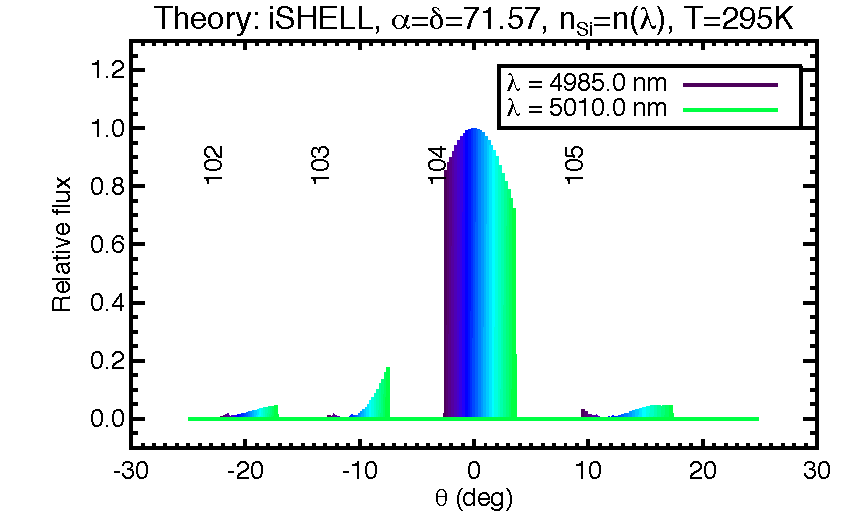
\psfig{file=ishell_Mband,height=3.8in,width=5.6in}}
\
\subfloat[Example L band blaze envelope]{\ 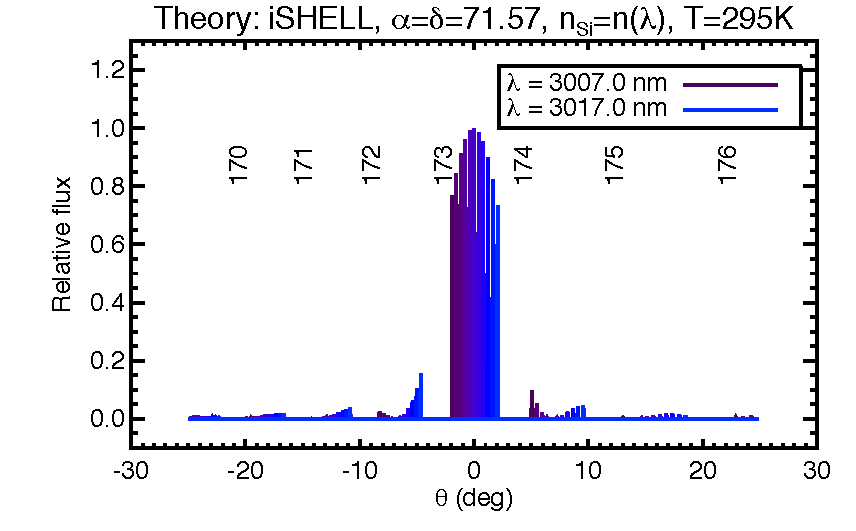
\psfig{file=ishell_Lband,height=3.8in,width=5.6in}}
\caption[Calculated $L-$ and $M-$ band blaze envelopes for iSHELL]{ L and M band blaze envelopes calculated from scalar diffraction theory in immersion.  The refractive index is based on the (cite XX) Sellmeier equations for Si at room temperature (T$=295$ K).}
\label{fig:LMbandcalc}
\end{center}
\end{figure}

\begin{figure}[htb] 
\begin{center}
\subfloat[Example K band blaze envelope]{\ 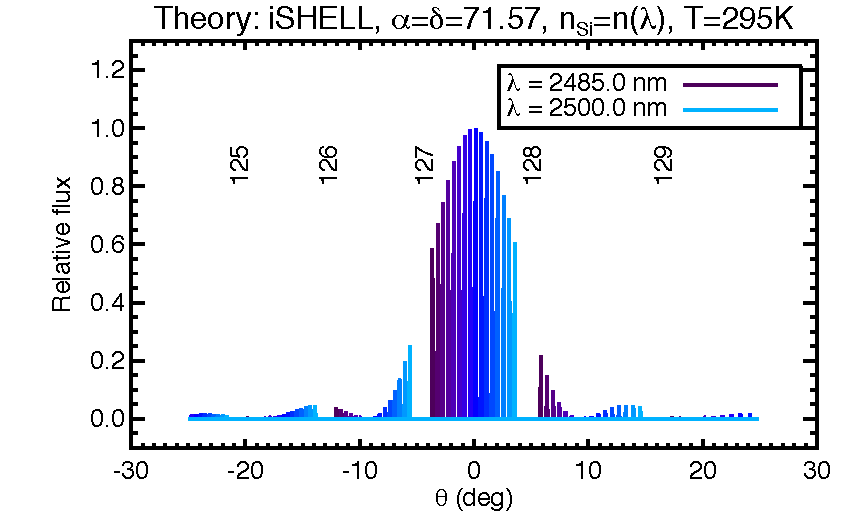
\psfig{file=ishell_Kband,height=3.8in,width=5.6in}}
\
\subfloat[Example J band blaze envelope]{\ 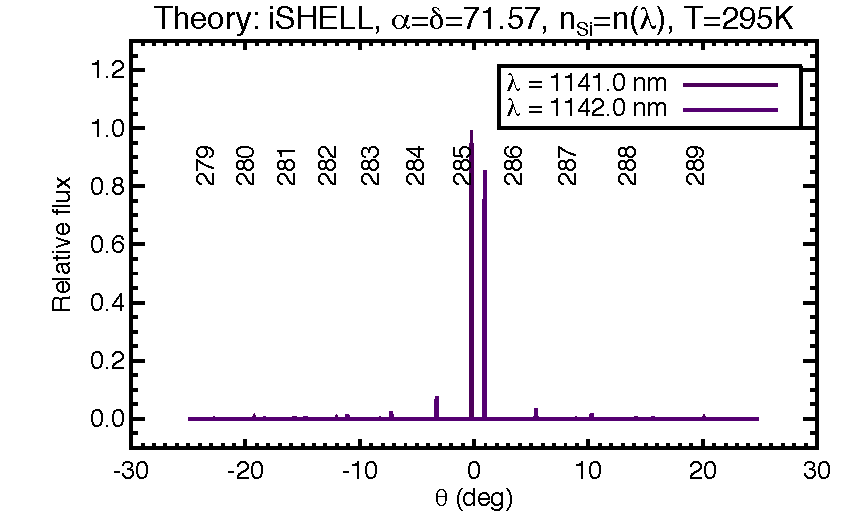
\psfig{file=ishell_Jband,height=3.8in,width=5.6in}}
\caption[Calculated $J-$ and $K-$ band blaze envelopes for iSHELL]{ J and K band blaze envelopes calculated from scalar diffraction theory in immersion.  The refractive index is based on the (cite XX) Sellmeier equations for Si at room temperature (T$=295$ K).}
\label{fig:JKbandcalc}
\end{center}
\end{figure}

\subsection{Optical evaluation}
Metrology is not possible in immersion until after the costly cost of cutting the Si pucks into prisms.  We perform optical metrology on the grating surface after KOH etching but before cutting.  The optical measurements have $\lambda=632$ nm, with $n=1$ for air.  We measure the PSF over a 25 mm beam in shallow images.  We construct deeper images by summing hundreds of read-noise limited CCD frames.
